
\documentclass[11pt,a4paper]{article}
\usepackage[margin=1in]{geometry}
\usepackage[utf8]{inputenc}
\usepackage{graphicx}


\usepackage{array}
\newcommand{\PreserveBackslash}[1]{\let\temp=\\#1\let\\=\temp}
\newcolumntype{C}[1]{>{\PreserveBackslash\centering}p{#1}}
\newcolumntype{R}[1]{>{\PreserveBackslash\raggedleft}p{#1}}
\newcolumntype{L}[1]{>{\PreserveBackslash\raggedright}p{#1}}


\title{MID PROJECT REPORT}
\author{Effat Jahan, ID: 18-38718-3}
\date{October 2021}

\begin{document}

\maketitle

\section{Abstract}
Handwritten digit recognition is the ability of a computer to recognize the human handwritten digits from different sources like images, papers, touch screens, etc. As handwriting differ from person to person. The goal of this project is to propose a \textbf{CNN} (\textit{Convolutional Neural Network}) model for \textbf{MNIST} dataset which will produce a accuracy over 98\%. Three different optimizers (\textbf{Adam, SGD, RMSprop}) will be used to get the best result possible.

\section{Introduction}

A Convolutional neural network (CNN) is a neural network that has one or more convolutional layers and are used mainly for image processing, classification, segmentation and also for other auto correlated data. CNNs have been used for understanding in Natural Language Processing (NLP) and speech recognition, although often for NLP Recurrent Neural Nets (RNNs) are used. Each convolutional layer contains a series of filters known as convolutional kernels. The filter is a matrix of integers that are used on a subset of the input pixel values, the same size as the kernel. Each pixel is multiplied by the corresponding value in the kernel, then the result is summed up for a single value for simplicity representing a grid cell, like a pixel, in the output channel/feature map.
\vspace{.5cm}
The \textbf{MNIST} (\textit{Modified National Institute of Standards and Technology}) database of handwritten digits, has a training set of 60,000 examples, and a test set of 10,000 examples. Each image contains 28*28 pixels where each pixel has a value from 0 to 255. I used 4 different layers including Conv2D layers, MaxPooling2D layers, Flatten layer and Dense layers in my model and used different optimizers to get the maximum accuracy. I have used two activation functions which includes \textit{ReLU} and \textit{Softmax} My model Summary is given below-
\begin{figure}[h]
\centering
    \includegraphics[scale=.6]{Images/fig1.jpg}
    \caption{Model Summary}
    \label{fig:my_label}
\end{figure}

Form this model summary we can see, I have used two conv2D layers and two MaxPooling2D layers. I have also used a flatten layer and two dense layer where one of them is the output layer

\section{Results}
The result of the model using different optimizers is given below -
\begin{table}[h!]
    \centering
    \begin{tabular}{|C{2cm}|C{2cm}|C{2cm}|C{2cm}|C{2cm}|C{2cm}|}
    \hline
       \textbf{Optimizer}  & \textbf{Train Accuracy} & \textbf{Train Loss} & \textbf{Validation Accuracy} &  \textbf{Validation Loss} & \textbf{Test Accuracy} \\
    \hline \hline
    Adam & 99.69\% & 0.89\% & 98.46\% & 6.95\% & 98.67 \% \\
    \hline
    SGD & 100\%  & 0.059\% &99.07\% & 4.64\% & 99.22\% \\
    \hline
    RMSprop & 99.99\%  & 0.026\% &99.14\% & 13.57\% & 99.17\% \\
    \hline
    \end{tabular}
\end{table}

The training and validation accuracy, training validation loss after using Adam optimizer is shown in the graph below-

\begin{figure}[h]
\centering
    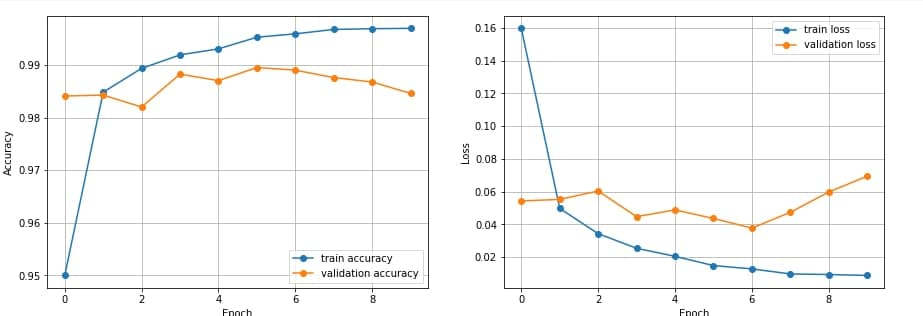
\includegraphics[scale=.6]{Images/Adam.jpg}
    \caption{Graph data of Adam Optimizer }
    \label{fig:my_label}
\end{figure}

The training and validation accuracy, training validation loss after using SGD optimizer is shown in the graph below-
\vspace{2cm}
\begin{figure}[h]
\centering
    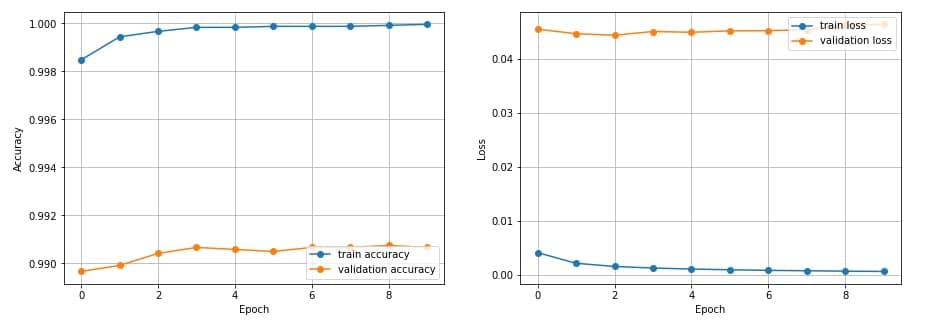
\includegraphics[scale=.6]{Images/SGD.jpg}
    \caption{Graph data of SGD Optimizer }
    \label{fig:my_label}
\end{figure}

\vspace{5cm}
The training and validation accuracy, training validation loss after using RMSprop optimizer is shown in the graph below-
\begin{figure}[h]
\centering
    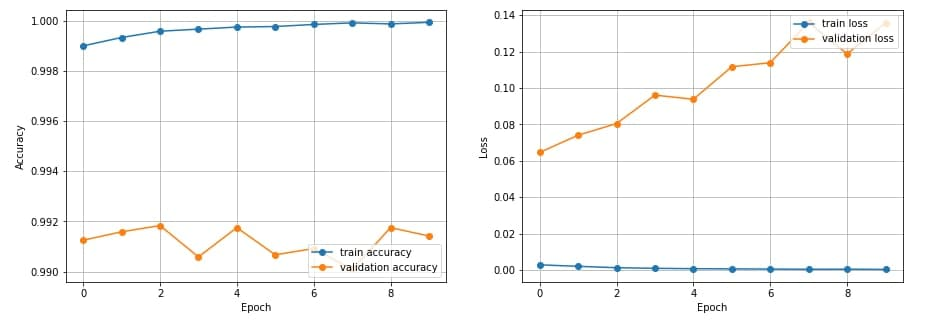
\includegraphics[scale=.6]{Images/RMSprop.jpg}
    \caption{Graph data of RMSprop Optimizer}
    \label{fig:my_label}
\end{figure}

\section{Discussion}
From the table data we can see that, on all three optimizer the proposed model accuracy is over 98\%.

While using Adam optimizer the training accuracy is 99.69\%, testing accuracy is 98.67\% and the validation accuracy is 98.46\%. In case of train loss and validation loss the data is 0.89\% and 6.95\% respectively.


While using SGD optimizer the training accuracy is 100\%, testing accuracy is 99.22\% and the validation accuracy is 99.07\%. In case of train loss and validation loss the data is 0.059\% and 4.64\% respectively.

While using RMSprop optimizer the training accuracy is 99.99\%, testing accuracy is 99.17\% and the validation accuracy is 99.14\%. In case of train loss and validation loss the data is 0.026\% and 13.57\% respectively.

Although, RMSprop closest value with validation accuracy and testing accuracy and had the lowest training loss It is not the best option as the validation loss is the highest. Considering all the data, it can be concluded that we can get the best output from this model by using SGD optimizer. It gives the highest training and testing accuracy with the lowest validation loss. 

\end{document}
